\documentclass{article}
\usepackage{graphicx} % Required for inserting images

\title{EECS510 Arithmetic Language Automaton}
\author{Jake Kice}
\date{November 2024}

\usepackage{tikz}
\usetikzlibrary{automata, positioning, arrows.meta, calc}
\tikzset{
->, node distance=3cm,
>={Latex[width=3mm,length=3mm]},
every  edge/.append style={thick, scale=1.8},
every state/.style={thick},
every  node/.append style={scale=1.4},
initial text=$ $, }

\tikzstyle{accepting}=[path picture={%
        \draw let
                \p1 = (path picture bounding box.east),
                \p2 = (path picture bounding box.center)
                in
                        (\p2) circle (\x1 - \x2 - 2pt); % adjust `2pt` here for clarity
}]

\begin{document}

\maketitle

%\section{Introduction}

    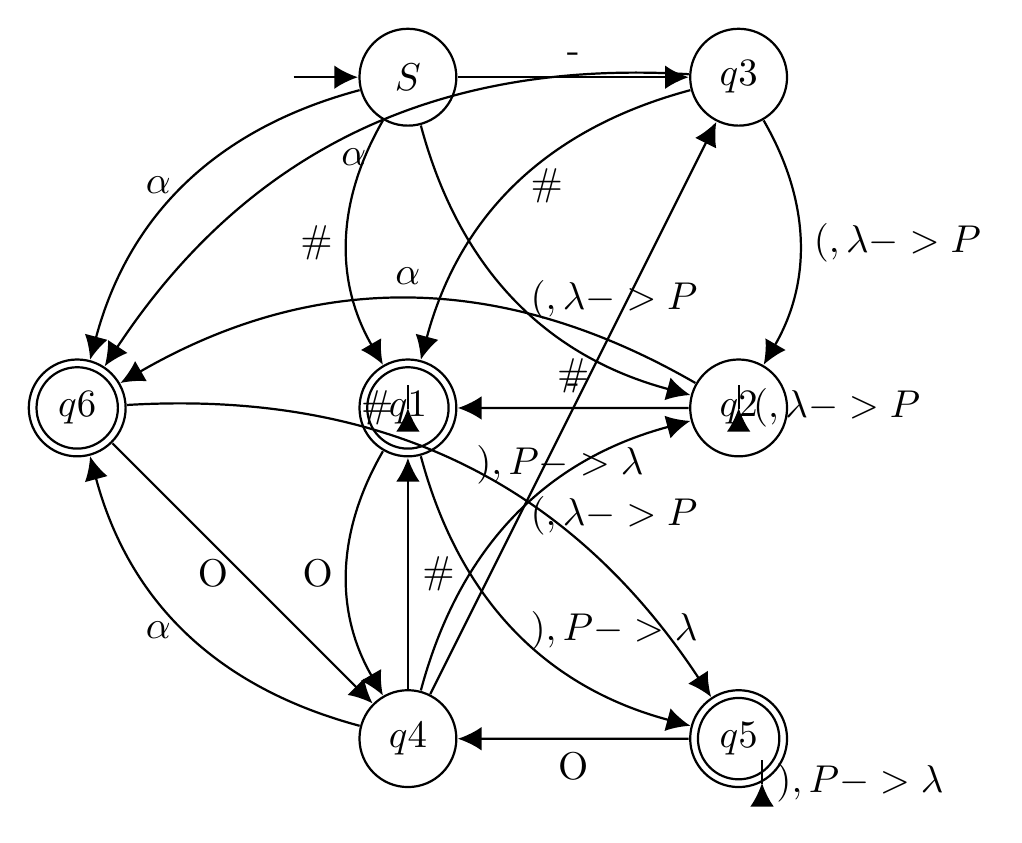
\begin{tikzpicture}
            \node[state,initial] (S) {$S$};
            \node[state, accepting, below of=S] (1) {$q1$};
            \node[state, accepting, left of=1] (6) {$q6$};
            \node[state, right of=1] (2) {$q2$};
            \node[state, right of=S] (3) {$q3$};
            \node[state, below of=1] (4) {$q4$};
            \node[state, accepting, right of=4] (5) {$q5$};

            % Transitions from S
            \draw (S) edge[bend right, left] node{$\#$} (1);
            \draw (S) edge[bend right, right] node{$(,\lambda->P$} (2);
            \draw (S) edge[above] node{-} (3);
            \draw (S) edge[bend right, left] node{$\alpha$} (6);

            % Transitions from 1
            \draw (1) edge[bend left, left] node{\#} (1);
            \draw (1) edge[bend right, left] node{O} (4);
            \draw (1) edge[bend right, right] node{$),P->\lambda$} (5);

            % Transitions from 2
            \draw (2) edge[above] node{$\#$} (1);
            \draw (2) edge[bend right, right] node{$(,\lambda->P$} (2);
            \draw (2) edge[bend right, above] node{$\alpha$} (6);

            % Transitions from 3
            \draw (3) edge[bend right, right] node{$\#$} (1);
            \draw (3) edge[bend left, right] node{$(,\lambda->P$} (2);
            \draw (3) edge[bend right, below] node{$\alpha$} (6);

            % Transitions from 4
            \draw (4) edge[right] node{$\#$} (1);
            \draw (4) edge[bend left, right] node{$(,\lambda->P$} (2);
            \draw (4) edge[above] node{-} (3);
            \draw (4) edge[bend left, left] node{$\alpha$} (6);

            % Transitions from 5
            \draw (5) edge[below] node{O} (4);
            \draw (5) edge[bend right, right] node{$),P->\lambda$} (5);

            % Transitions from 6
            \draw (6) edge[left] node{O} (4);
            \draw (6) edge[bend left, right] node{$),P->\lambda$} (5);
            
     \end{tikzpicture}

\end{document}
